\documentclass{sig-alternate}
\usepackage{algorithm}
\usepackage{algorithmic}
\usepackage{url}
\usepackage{subfigure}

\pdfpagewidth 8.5in
\pdfpageheight 11in

\title{Crowdy: Social Crowd Visualization}

\numberofauthors{1} 
\author{
    \alignauthor Jeffrey McGee, Zhiyuan Cheng, Chiao-Fang Hsu, Pratheek
    Kumar Akireddy \\
    \affaddr{Department of Computer Science and Engineering, Texas A\&M
    University} \\
    \affaddr{ College Station, TX 77845 USA} \\
    \email{jeffamcgee@gmail.com, zcheng@cse.tamu.edu, drakihsu@cse.tamu.edu,
    pka293@cse.tamu.edu}
} 
\begin{document}

\maketitle
\begin{abstract}
Microblogging systems have provided society with a more transparent channel
for information distribution. Each individual is empowered to spread news
and build their social network. With the freedom of information generation,
the issue now is identifying, organizing, and visualizing useful information.
For this project, we want to design an user interface that takes
both usefulness and usability into consideration. Our system will
adapt to different types of users and display the crowds that form in a specific
period of time as well as the topics discussed by the crowd from Twitter. The
interface should both optimize the user experience and system speed. For
evaluation, we will design a user study to
test the efficiency, effectiveness, and satisfaction of this system to our
potential users.
\end{abstract}

\category{H.5.1}{Information Interfaces and Presentation}{Multimedia
Information Systems}[video]
\category{H.5.3}{Group and Organization Interfaces}[collaborative computing,
computer-supported cooperative work]
\category{H.5.4}{Hypertext/Hypermedia}[architecture]

\terms{Design, Experimentation, Human Factors}

\keywords{interface, crowd, Twitter}

\section{Introduction}
Along with the rise of real-time social web, the power of information
distribution is no longer limited to the small set of news media but the
massive amount of ordinary individuals. Websites like Digg and Reddit provide
a news aggregation platform that filter and display interesting news pieces
recommended by other users; social media object sharing sites like Youtube and
Flickr let users upload and browse videos and images; microblogging systems,
like Twitter and Buzz, enable every user to host a broadcasting station of
their own; last but not least, Facebook allows users to build their own
social network and share their everyday experience with their friends.
Thus, there is a demand for services that
exploit these massive sources of data. People are looking for a new
generation of applications for monitoring, analyzing, and distilling
information from the prospective web of real-time content that reflects the
current activity of the web's participants. The shift toward fresh web content
can be seen in the growing interest in mining large-scale social media for
information discovery and brand management, for intelligence analysis by the
government and state media, and in identifying and disseminating disaster and
emergency-related information.

Comparing with the traditional web information applications that apply
expensive off-line analysis of web data, the new generation of real-time web
applications must be able to consume, process and display the massive amounts
of data on-the-fly. In this project, we look particular into Twitter, a
microblogging platform. We want to provide users a manageable
exploratory interface that displays the crowds and their associated
participants/content at each time period.  We define a ``crowd'' to be a
potentially short-lived ad-hoc collection of users.  There are several ways to
identify crowds: users who message each other, users who are nearby, and users
who use similar terms. In Twitter, there are potentially 100s of millions of
active users inserting new messages into the system at a high rate. With
existing algorithm and architecture built by our lab in the backend, our goal
is to reveal the ad-hoc crowds of users that reflect the real-time interests
and highly-temporal group affiliations in a clear and manageable fashion.

Even though our current data is from Twitter, we expect the system to be useful
to users who are not familiar with Twitter. In fact, our system can be of
useful to several types of users with different purpose in mind.

\subsubsection{How Might We Help}
Apart from the original Twitter interface that provides only a local view of
the most current tweets issued by each user's followee or some local trending
topics, our final system should be able to aggregate the data to find global,
regional, and local phenomenons. The final product is also adjustable that fit
into different expertise and purpose of usage based on the role of the users.

\subsection{Conceptual Model}
The conceptual model of our system is a tool for finding patterns, trends, and
communities. The interface displays groups of people who are talking with each
other, puts their conversation on a map, and finds important words in the
conversation. Users will expect different types of filtering options such as
filtering by area(geo-feature), by time(timeline snapshot), by
keyword(free-text, hashtag) or by the expecting property of the crowds(the
longest living crowd, the most engaging crowd). The default view of the system
is a set of global crowds discovered recently.


\subsection{User}
To better design our system interface, we want to understand our potential
users. For different kinds of users, there exhibits different patterns of
properties like the frequency of usage, the level of experience, the behavior
tendency and the tuning options availability.
\begin{itemize}
    \item Analyst: Government or media analyst are experts in information
    trending and market research. They use the system regularly with the
    frequency between once per day to once per month depending on the urgency
    of the monitoring task itself. They would like to have a customized interface
    that is able to apply a variety of filters on the fly. While they are 
    investigating the data using our system, they are likely to be writing a
    report.

    \item Twitter Users: Twitter users who already have familiarity with the
    Twitter world can use our system to learn about crowds
    and hot-topics. The may use it regularly or occasionally. They adopt our
    system to assist their twittering experience. They might not devote a large
    amount of time and effort but just want a quick and fresh view of the
    current trend. For this purpose, we should provide a simple and
    personalized content display with some easy filtering options.

    \item Regular People: regular users with no Twitter experience will use
    our system as a window to gain an idea of what is currently happening
    in the Twitter world. To satisfy their curiosity without personalized
    history to learn from, we provide a global trend as the first look.
    Ideally, the users will come back and build a history profile so we can
    customize the display in a long run. people could use it just once or, if
    they like the system, several times per day.

    \item Business People - corporate employees are particularly interested in
    their own product or company. Like the analysts, they are asked to perform
    the trending survey in a regular basis. They are trained in finding
    information related to their product. They use our system to find the
    opinion from the general users. They also study their competitors in a hope
    to improve their own. For this type of user, we can do highly customized
    interface to pre-filter the crowds to display. We may also prepare a set of
    templates so the business people with no computer science knowledge can
    easily drag-and-drop views related to their competitors and their own
    business side by side.

\end{itemize}

\subsection{Cognitive Issue}
Some cognitive issues we need to consider include the other activities our
users might be engaging in simultaneously. For example, the Twitter user might
be browsing Twitter and plan to use our system to understand the crowds that
talk about a certain keyword of interest. Another situation can be finding some
interesting topics while playing with our system and decide to do search to
read the related news article from Google or NY Times. Or, our users may
discover an exciting crowd/topic and eager to share this discovery to his
friends on the social websites(Twitter, Facebook, etc). That is to say, we does
not expect our user to keep 100\% focus on interacting with the system. We need
to provide mechanisms for tip reminding of behavior history. 

In addition, with the nature of the temporal massive data, we do not expect our
users to remember where to find the crowd/topic of interest that the user just
encountered. We want to provide a Workspace panel so to release the stress on
the memory requirement from the user.

\section{Related Work}
There has been some work into understanding how communities of users interact
on social networks. Along with working on understanding microblogging usage and
communities\cite{java2007we}, the main author - Akshay Java was one of the
first few who dealt with the measurement of the usage and nature of communities
in microblogging. In his latter study\cite{java2008mining}, he presented his
observations of the microblogging phenomena and user intentions by studying the
content, topological and geographical properties of such communities. He found
that microblogging provides users with a more immediate form of communication
to talk about their daily activities and to seek or share information.

When it comes to visualization of social crowds, a tool which has
similar objectives to ours is
Vizster\cite{heer2005vizster}. It is a visualization system for playful
end-user exploration and navigation of large-scale online social networks. The
design builds upon familiar node-link network layouts to contribute techniques
for exploring connectivity in large graph structures, supporting visual search
and analysis, and automatically identifying and visualizing community
structures. The system facilitates discovery of people, connections,
and communities to promote increased awareness of community structure and
information exposure, while maintaining a fun and socially engaged online
space. The creators of the tool were interested in crafting techniques for the
situated exploration and visual analysis of large graph structures by a
specific end-user population.

Another related study was on how web-based retrieval from Twitter can be used
as knowledge base\cite{cheong2009integrating} which shows that the
visualization system we try to attempt can be helpful. Marc Cheong et al. in
this study tried to analyze demographics of the authors of Twitter messages and
attempt to map a Twitter trend into what's going on in the real world. Their
findings reveal a pattern behind trends on Twitter, and trying to evolve
through visualization methods.  Their findings also enable us to understand the
underlying characteristics behind the ``trend setters'', providing us a new
perspective on the contributors of a trend.

Identifying highly dynamic ad-hoc collections of users what we refer to as
crowds in massive social messaging systems like Twitter and Facebook is
important\cite{kamath2010identifying}. K. Y. Kamath et al. in the study have a
salient feature of the proposed approach as an efficient locality-based
clustering approach for identifying crowds of users in near real-time compared
to more heavyweight static clustering algorithm. The study consisted of 711,612
users and 61.3 million messages, which show how the proposed approach can
efficiently and effectively identify Twitter-based crowds.

In the other study based on the previous one, K. Y. Kamath et
al\cite{kamath2011transient}, they add another salient feature - a novel crowd
tracking and evolution approach for linking crowds across time periods. Unlike
the more static and long-lived group-based membership offered on many social
networks their goal is to support the discovery of organic and highly-temporal
group affiliation, which they refer to as ``transient crowds''. A transient
crowd according to them is a potentially short-lived ad-hoc collection of users
bound together by some common thread – which can be communication-based,
location-based or interest based. We are inspired by this idea of formation and
detection of crowds. We try to implement detection of crowd in “Crowdy” in a
similar fashion.

\section{Interface Design}

\begin{figure*}[t]
\centering
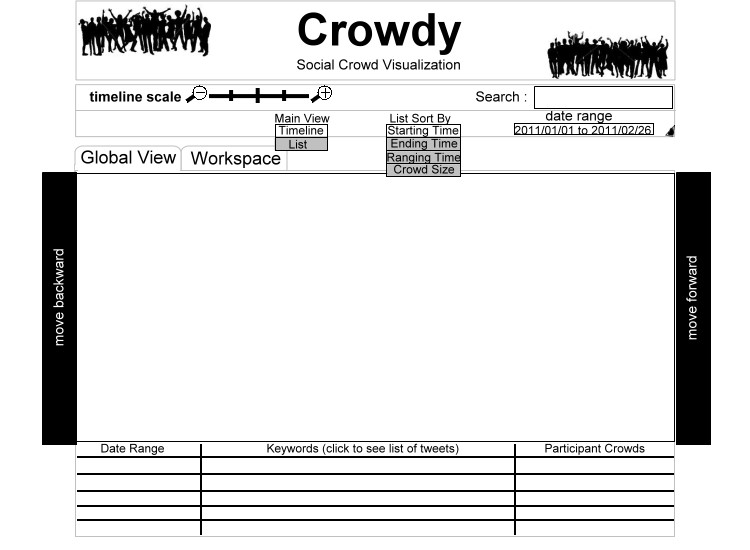
\includegraphics[width=400pt]{img/UIdesign.eps}
\caption{Crowdy User Interface Design}
\label{fig:UIdesign}
\end{figure*}

Figure \ref{fig:UIdesign} shows an outline of the prototype. We want to provide
the user with a simple and flexible interface to maximize their options for
exploring while minimizing their memory overhead. Existing web applications
show that the most general task should be the main focus and the other
available options may be placed on the side or hidden according to their
frequency of usage. Since the primary function of our system is to visualize
the Crowds emerged over time, the crowd display window is our
first priority. In the crowd display window, we
consider the needs of personalization for our potential users(e.g. Analyst).
There is a global view panel and a personal workspace panel. The personal
workspace panel distinguishes from the global view panel in a way that it only
shows the set of crowds marked by the user when exploring in the global view
panel. We have tabs to help our users quickly and easily transit between these
two views. Inside each view, we need to decide the best format to condense
a massive amount of data. Each crowd has metadata associated with it such as
starting and ending time, crowd participants, topics, tweets,
location data, etc. To effectively organize these properties to assist quick
and convenient retrieval by the user, we consider these two formats: timeline
and list. For both view panels, these two formats are included but sized
unequally. The size is adjustable(in the option panel) according to the user's
need. Generally, ``timeline'' is more suitable for overview a large number of
crowds while ``list'' is better for investigating details in a smaller set of crowds. We
also provide several filtering options for both timeline and list format in the
option panel. Some detailed components in these three panels are listed below.

\begin{itemize}
    \item \textit{Global View Panel} : The global view shows the global crowds
    in different format. When a crowded is marked by the user, a flag will be
    placed in front of each crowd item in each format.

    \begin{itemize}
        \item Timeline format displays the evolution of each crowd.
        First of all, a crowd is shown as a line from the starting time
        to the ending time. The size of the participants over time is
        indicated by color(e.g., small-large-medium $\longrightarrow$
        green-red-blue). The top three keywords that describe the topic of
        the crowd are displayed explicitly on the timeline along with
        the crowd line. Extra information about the crowd can be viewed
        in the pop up box when the user clicks on the crowd line.
        \item List format displays each crowd with some specific
        sorting order. The default sorting order is by the starting
        time. Some other available sorting functions include the
        ending time, the size of crowds and the ranging time. In the
        list format, crowds are displayed explicitly in three columns:
        time period, keywords and some of the participants. The latter
        two columns are clickable. After clicked, it will show the list
        of tweets and the full set of participants in a pop up window
        form.
    \end{itemize}

    \item \textit{Personal Workspace Panel} : Similar as the Global View Panel
    but with only the set of crowds marked by the user in the Global View
    Panel.
    \item \textit{Filter Option Panel} : This panel explicitly displays a set of
    the most frequently used filtering options such as search and timeline scaling.
    We also provide the user with flexibility to adjust the default
    settings we provided such as the primary display format in the View
    Panel, list sorting function and time period filtering. Other filtering
    options are hidden and can be expanded with a click on the right bottom corner
    of the Panel.
\end{itemize}

\section{Implementation}
The system is designed to run in a user's web browser.
As a result, we choose to use some fairly standard web tools to implement the system.
The system that we are building the user interface on top of exposes a RESTful API.
To retrieve data, our system makes an HTTP GET request to the server.
The server returns data in the JSON format, which is easy to decode in Javascript.

CherryPy
Jinja

jQuery
Simile Timeline
Google Maps API

\section{Evaluation}

\section{CONCLUSIONS}

\section{FUTURE WORK}

\bibliographystyle{abbrv}
\bibliography{reference} 
\end{document}
